\documentclass{sig-alternate-10pt}
%\documentclass[letterpaper,11pt]{article}
\usepackage{url}
%\usepackage{usenix,epsfig,endnotes}
%\usepackage{fullpage} 
\setlength{\textheight}{9.5in}
%\setlength{\textwidth}{6.75in}
%\setlength{\oddsidemargin}{-.125in}
\usepackage{graphicx}
\usepackage{enumerate}
%\usepackage{subfigure}
%\usepackage{ifpdf}
%\usepackage{multicol}
%\usepackage{amsmath, amssymb, amsthm}
%\usepackage{rotating}
%\onehalfspacing
%\newcommand{\tbd}[1]{[{\bf{#1}}]}
\newcommand{\tbd}[1]{}
\newcommand{\ie}{{\it i.e.}}
\newcommand{\eg}{{\it e.g.}}
\newcommand{\etc}{{\it etc.}}
\newcommand{\eat}[1]{}
%\renewcommand\bibname{}

%\setlength\topmargin{0in}
%\usepackage{verbatim}
%\usepackage[compact]{titlesec}
%\usepackage[small]{caption}
\usepackage{times}

\title{Correspondence Checking for Computer Networks \\
\Large{CS 263 Project Proposal \vspace{-25pt}}}

\author{Colin Scott\thanks{In collaboration with Andi
Wundsam and Scott Shenker}\vspace{-15pt}}

%        \begin{multicols}{2}{{\it Draft - Please do not distribute.}}\\
        
%\author{Paper \#69, 14 Pages}
\date{}
\begin{document}
    \maketitle
    \thispagestyle{empty}
\section{Background}

\subsection{Model}

Computer networks can be represented as directed graphs:
\begin{align*}
G = (V, E)
\end{align*}

Forwarding elements are represented as internal vertices:
\begin{align*}
V_{fwd} = \{ v \in V |\text{ } degree(v) > 1 \}
\end{align*}

End-hosts are represented as edge vertices:
\begin{align*}
V_{host} = \{ v \in V |\text{ } degree(v) = 1 \}
\end{align*}

End-hosts send and receive packets. A packet's source and destination,
among other information, is encoded in the packet's header:
\begin{align*}
h \in \{0,1\}^L = H
\end{align*}
where $L$ is the number of bits in
the header \cite{HeaderSpace}.

Upon receiving a packet, forwarding elements apply a transformation function
\footnote{We assume unicast forwarding for the purposes of this proposal}:
\begin{align*}
T: (H \times E) \rightarrow (H \times E_{\emptyset})
\end{align*}
Note that forwarding elements may rewrite fields of a packet header before passing it along.
Forwarding elements may also drop packets, in which case $T(.) = (.,\{\})$.

We use $`\Psi`$ to denote the collection of all transfer functions present in
the network at a particular point in time.

In this model, network traversal is simply a composition of transformation
functions. For example, if a header $h$ enters the network through edge
$e$, its state after $k$ hops will be:
\begin{align*}
\Phi^k(h,e) = \Psi(\Psi(\dots \Psi(h,e)\dots))
\end{align*}

Only end-hosts can insert new packets into the network \footnote{We ignore
control and diagnostic traffic for the purposes of this proposal}. The access links
of end-hosts are therefore the only entry and exit points for packets:
\begin{align*}
E_{access} = \{ (v_1,v_2) \in E |\text{ } v_1 \in V_{host} \vee v_2 \in V_{host} \}
\end{align*}

The externally visible behavior of the network is expressed as a relation between
packets originating from end-hosts and the packets' final locations:
\begin{align*}
\Omega: (H \times E_{access}) \rightarrow (H \times E_{\emptyset}) \\
\Omega(h,e) = \Phi^{\infty}(h,e)
\end{align*}

\subsection{Software-defined Networks}

Software-defined Networking (SDN) is a paradigm for controlling network behavior.
The SDN platform maintains a data-structure representing the global state of the
network. We refer to this data-structure as the `view`:
\begin{align*}
G^{view} = (V^{view},E^{view})
\end{align*}

Control programs running on top of the SDN platform configure the network by
defining $\Psi^{view}$. The role of the platform is then to map $\Psi^{view}$ to
routing entries in the underlying forwarding elements of the
physical network. The physical network is also a graph:
\begin{align*}
G^{physical} = (V^{physical}, E^{physical}) 
\end{align*}

Note that the mapping between $G^{view}$ and $G^{physical}$ is not
necessarily one-to-one; the SDN platform may virtualize the view
such that a single member of $V_{fwd}^{view}$ maps to multiple members of
$V_{fwd}^{physical}$.

A common pattern is to map a single forwarding element $v \in V_{fwd}^{view}$ to
an entire physical network $V_{fwd}^{physical}$. Figure \ref{fig:view_and_physical}
depicts an example. In the example, $V_{fwd}^{view} = \{ Switch \}$, and
$Switch$ maps onto:
\begin{align*}
V_{fwd}^{physical} = \{ vswitch_1, vswitch_2, vswitch_3, \\
vswitch_4, TOR_1 TOR_2, Gateway \}
\end{align*}

\begin{figure}[t]
\hspace{-10pt}
\begin{tabular}{c}
    $G^{view}$ \\
    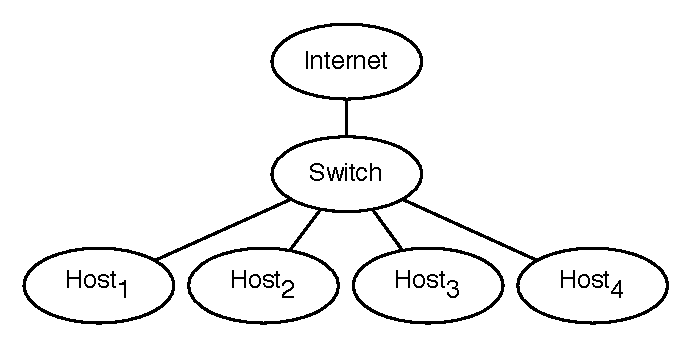
\includegraphics[width=3.25in]{../diagrams/necula_views/app_view.pdf}  \\
    $G^{physical}$ \\
    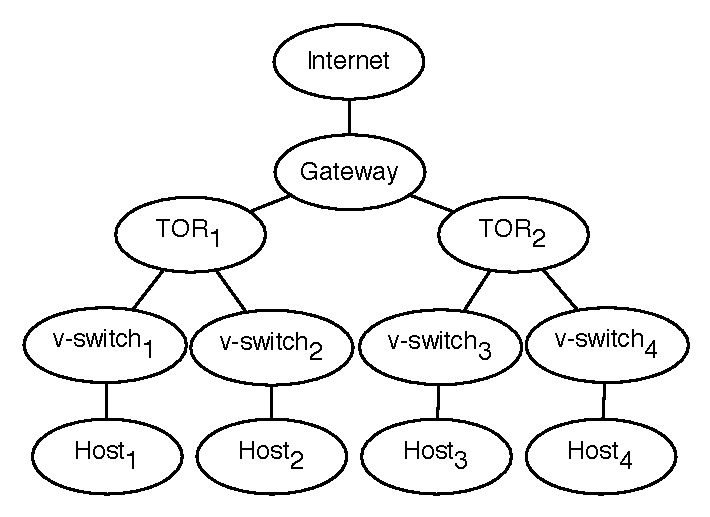
\includegraphics[width=3.25in]{../diagrams/necula_views/physical_view.pdf}
\end{tabular}
\caption[]{\label{fig:view_and_physical} Example correspondence between
$G^{view}$ and $G^{physical}$. In the view a single switch connects 
four hosts and the rest of the Internet (modeled as a single vertex).
This single switch is mapped onto four v-switches, two top-of-rack switches 
and one gatway router in the physical network.}
\end{figure}

As we will see later on, it is important to note that there is still a one-to-one correspondence
between $V_{host}^{view}$ and $V_{host}^{physical}$, as well as between
$E_{access}^{view}$ and $E_{access}^{physical}$.

\section{Problem Statement}

It should always be the case that there is a correpondence between
$\Omega^{view}$ and $\Omega^{physical}$, {\it viz.}:
\begin{align*}
\forall_{h} \forall_{e \in E_{access}^{view}} \Omega^{view}(h,e) =
\Omega^{physical}(encap(h),\hat{e}) 
\end{align*}
where $encap$ is a function from packets in $G^{view}$ to packets in
$G^{physical}$, and $e \sim \hat{e} \in E_{access}^{physical}$.

In practice however, there are often miscorrespondences between the two. Some
of these miscorrespondences are innocuous; networks are distributed systems,
and there are inevitable delays between updates in $G^{view}$ and the
corresponding changes in $G^{physical}$. Other miscorrespondences are
due to critical bugs in the SDN platform. In general, the SDN platform is a
highly complex piece of software; it must deal with hardware-faults,
communication delays, and complex mapping functions  between $G^{view}$ and
$G^{physical}$. Moreover, production networks may contain  $10's$ of thousands of
forwarding devices. In such an environment, the control program must be
replicated across multiple servers to handle the load and ensure
fault-tolerance. The SDN platform must ensure that $G^{view}$ remains consistent
between all replicas, despite server failures, communication delays, and
message re-orderings.

\section{Proposal}

I propose to design and build a mechanism for checking 
correspondence between $\Omega^{view}$ and $\Omega^{physical}$.
I plan to leverage techniques from model-checking and symbolic execution \cite{symbolicmodel}.
In particular, my initial design is roughly as follows:
\begin{enumerate}[i.]
\item Take a distributed snapshot of $G^{physical}$ \cite{distributedsnapshots}
\item Translate the routing tables of $V_{fwd}^{physical}$ into tranformation
functions $\Psi^{physical}$
\item Feed symbolic packets $h_s$ through each access link $e \in E_{access}$
\item Track the progress of $h_s$ through the network, thereby computing
$\Omega^{view}$
\item Do the same for $G^{view}$
\item Identify counterexamples:
\begin{align*}
 \{ (h,e) |\text{ } h \in H, e \in E^{view}_{access} \sim
 E^{physical}_{access}, \\
 \Omega^{view}(h,e) \neq  \Omega^{physical}(h,e) \}
\end{align*}
\end{enumerate}

I will implement my correspondence checker within the POX control platform
\cite{POX}.
I plan to submit this work, along with other aspects of my SDN debugger, to
OSDI 2012.

\scriptsize
\bibliographystyle{abbrv}
\bibliography{bib}

%\input{appendix}
\end{document}
